\chapter{Conceptual Design}

\section{Line Cutting Methods}

\subsection{Electro-mechanical mechanism}
\subsubsection{Servomotor Actuator}\label{servo-actuator}
A servo motor is a rotary actuator that allows for precise control of the angular position. It consists of a motor coupled to a sensor for position feedback and a drive unit. Hobby-grade servomotors are cheap and available in a variety of sizes.\cite{servo-motor}

For the servomotor actuated concept, the rotary movement of the servo needs to be translated into a linear movement to release the reefing line. The reefing line is attached to both ends of the mechanism. Figure \ref{fig:servo} shows a concept where only one side of the reefing line can be released. The loop in the reefing line is released when the servomotor is actuated, moving the rod down. A concept with two servos to release both loops is feasible, although with the downside of increased weight and size. 

\begin{figure}[h!]
	\centering
	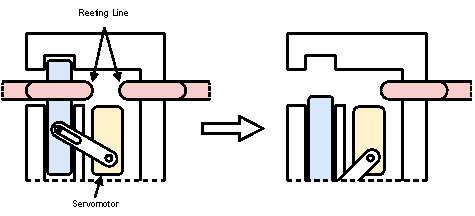
\includegraphics[width=\textwidth]{images/servo}
	\caption{Servomotor release mechanism concept}
	\label{fig:servo}
\end{figure}

\newpage

One of the main issues with this design is the complexity of the mechanical system, and the size and weight constrain. In addition, the loops in the reefing line could entangle with a reefing ring, resulting in a partial opening of the parachute. 

\subsubsection{Linear Solenoid Actuator}
Linear solenoids are electro-mechanical devices that generate a uniform magnetic field when an electric current is applied. They are composed of a coil of wire wrapped around a moveable metal core. The main advantage of solenoid actuators is that the movement is linear; therefore, they can be easily deployed to release a hook.\cite{solenoid-actuator}

The solenoid actuator concept is very similar to the servo actuated release mechanism. As shown in Figure \ref{fig:solenoid}, two solenoid actuators hold on to both ends of the reefing line. The solenoids pull the metal rods down when powered, releasing the reefing line. 

\begin{figure}[h!]
	\centering
	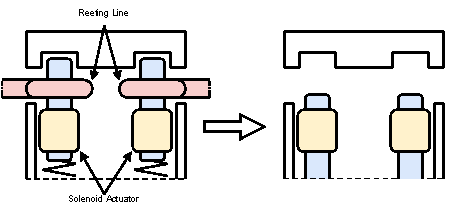
\includegraphics[width=\textwidth]{images/solenoid}
	\caption{Solenoid release mechanism concept (side view, parallel to reefing line)}
	\label{fig:solenoid}
\end{figure}

When solenoids of small size were tried, it was immediately found that they had a meager force. Releasing a reefing line under tension required very large and heavy actuators. Moreover, the same issue described in the servomotor actuated concept also applies to this design. The loops in the reefing line can entangle with reefing rings, preventing the parachute from opening. 

\subsubsection{Continuous Disreefing}
Continous disreefing was briefly considered. In this concept, it was thought of to use a brushless DC motor. The reefing line would be rolled on a spool and then gradually released with the motor. Brushless DC motors can be operated in a constant torque mode, resulting in a very smooth and controlled opening of the parachute canopy.

Some of the significant drawbacks of such a system are complexity, size, and weight.

\newpage

\subsection{Pyrotechnic cutter}
Pyrotechnic cutters were specially designed for this application. They consist of a pyrotechnic charge, a cutting blade, and a piston. On ignition of the pyrotechnic charge, pressure builds up behind the piston, pushing it forward into the reefing line. Severed by the blades, the reefing line is released. Their high reliability and cutting force make them excellent for safety-critical applications. Because of that, pyrotechnic cutters are the industry standard for space and military applications.\cite[Chapter~6.5]{parachute-design}   

\begin{figure}[h!]
	\centering
	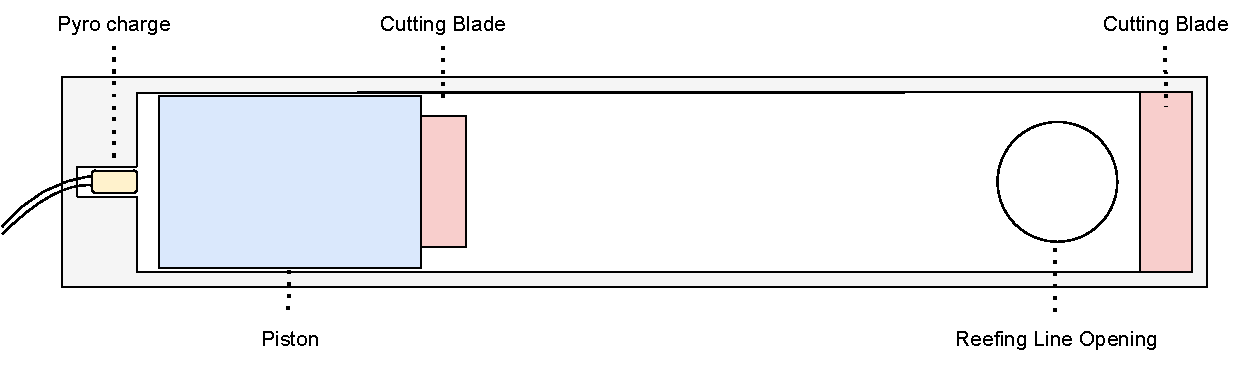
\includegraphics[width=\textwidth]{images/pyro-cutter}
	\caption{Illustration of pyrotechnic line cutter}
	\label{fig:pyro-cutter}
\end{figure}

  Developing a pyrotechnic cutter from scratch was never considered as the author lacks the knowledge of mechanical design. Thus some commercial options were investigated. The Mako Line Cutter from Tinder Rocketry turned out to be a good match for the application. The low weight, high power, and low price are some of the system's advantages. The cutter is advertised to cut paracord, zip ties, and copper wires. Unfortunately, pyrotechnic line cutters are labor- and time-intensive to set up. After every deployment, the igniter, black powder, and a sealing O-ring must be replaced. A turnaround time of fewer than 24 hours is impossible, as epoxy, used to seal the igniter cables, needs to cure overnight.

\begin{figure}[h!]
	\centering
	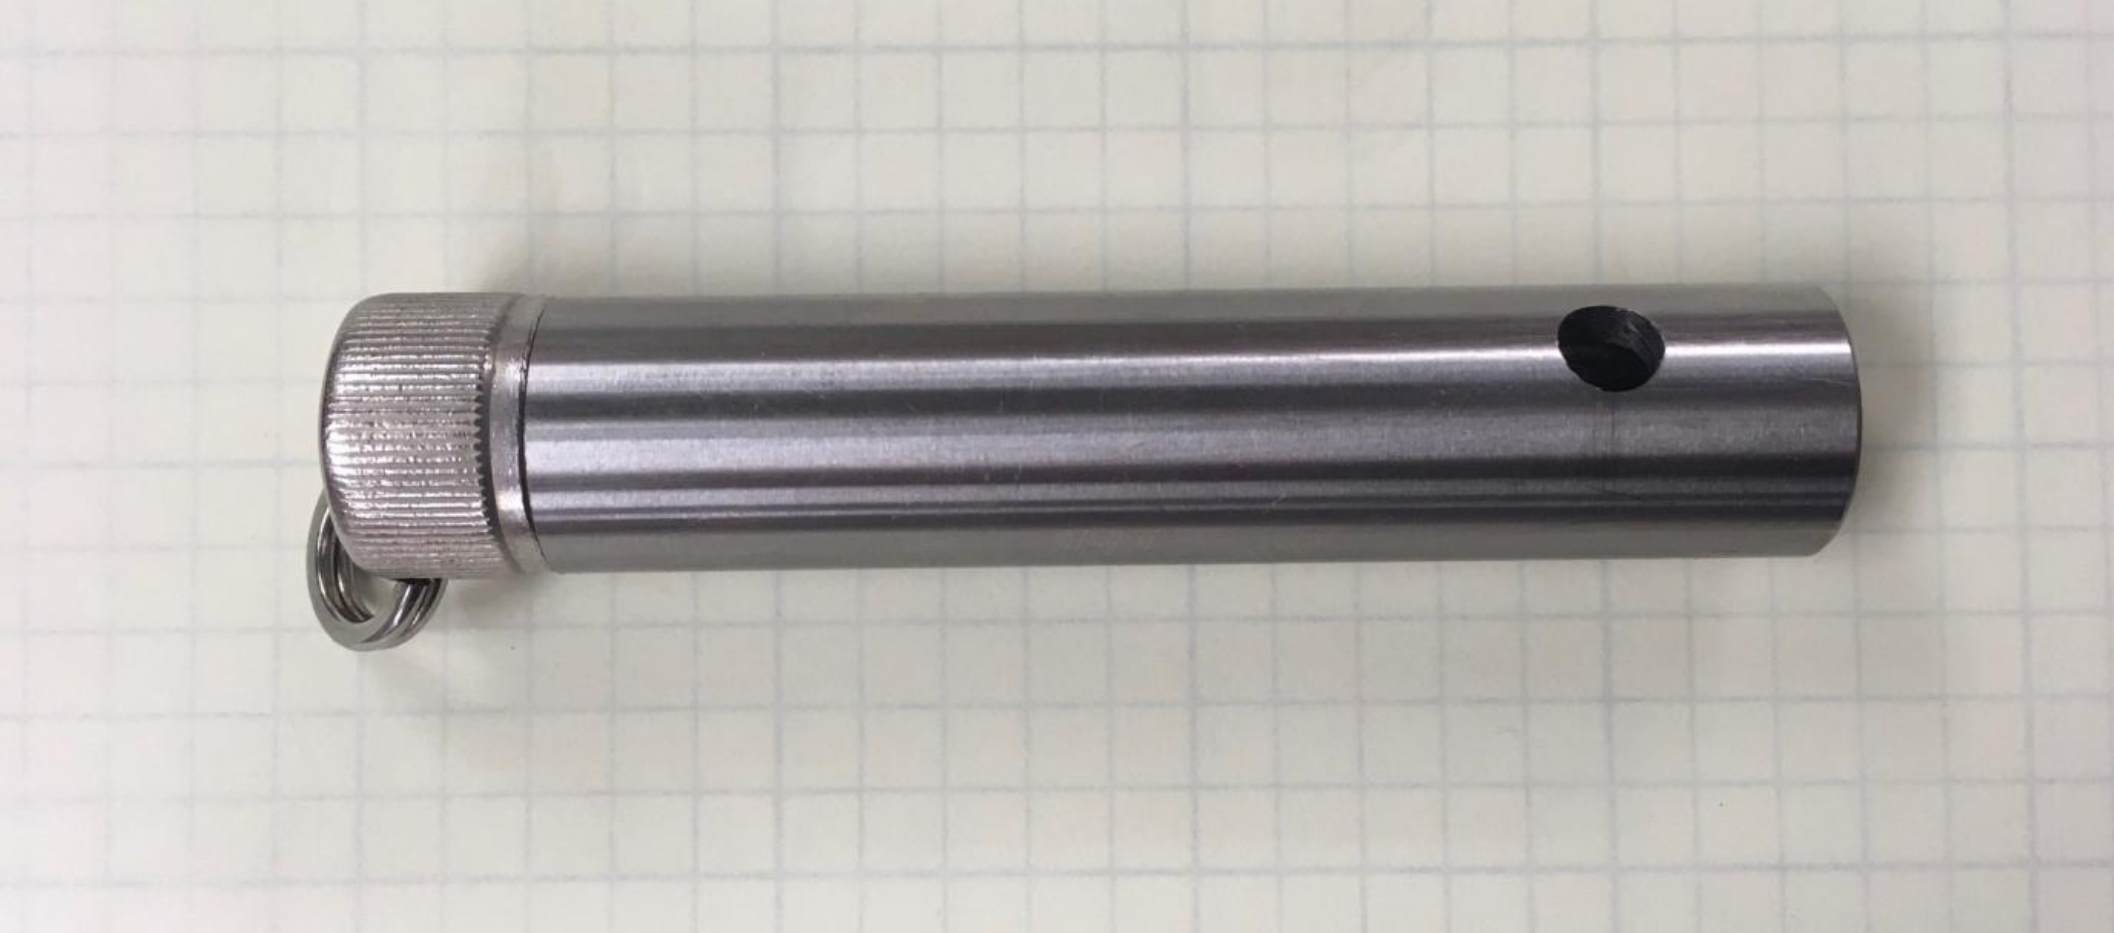
\includegraphics[width=13cm]{images/tinder-rocketry}
	\caption{Make Line Cutter from Tinder Rocketry}
	\caption*{\textbf{Source:} Mako User Instruction Manual  \cite{mako-user-instuction}}
	\label{fig:mako-cutter}
\end{figure}

\newpage


\subsection{Thermal cutter}
During the conceptual design phase, it was identified that the most commonly used parachute lines have a low melting point, making them suitable for thermal separation. Table \ref{tab:thermal-properties} shows the thermal properties of different rope materials.

\begin{table}[h]
    \centering
    \begin{tabular}{ | l | c |}
      \hline
      \textbf{Material}             & \textbf{Melting Point}    \\ \hline
      High Modulus Polyethylene     & 140-150$^\circ$C          \\ \hline
      High Modulus Polyester        & 280-330$^\circ$C          \\ \hline
      Para-aramid                   & 500$^\circ$C $^1$         \\ \hline
      PBO                           & 650$^\circ$C $^1$         \\ \hline
      Polyester                     & 225-240$^\circ$C          \\ \hline
      Polyamide                     & 215-260$^\circ$C          \\ \hline
      Polypropylene                 & 165-175$^\circ$C          \\ \hline
    \end{tabular}
    \caption{\label{tab:thermal-properties}Melting point of commonly used rope materials}
    \caption*{\textbf{Source:} Barry: Technical Properties of Synthetic Fibres \cite{fibers}}
\end{table}
\begin{footnotesize}
        {$1$ Carbonizes before it burns or melts}
\end{footnotesize}

As shown in Table \ref{tab:thermal-properties} all but two of the most commonly used rope materials are suitable for a thermal reefing system. Para-aramid, often branded under the name \textit{Kevlar} is a widespread parachute line material for space missions but is rarely seen in more miniature parachutes. Paracord, designed initially for use as parachute suspension lines, is a lightweight polyamide rope. Due to its strength, elasticity, and comparatively low melting point, it is well suited for a thermal line cutting system.


\subsubsection{Nichrome Wire}\label{nichrome-wire}
Nichrome is widely used in electric heating elements because of its resistance to oxidation, stability at high temperatures, and resistance to the flow of electrons.\cite{nichrome} With a melting point of 1350\,$^{\circ}C$, it can be used to burn through almost all types of ropes. One of the issues with using just a wire is that the rope needs to be in constant contact with the nichrome wire while still being able to move around freely. Therefore, a spring-loaded mechanism was thought of, pushing the nichrome wire against the rope and the case wall. Two posts made out of metal span the nichrome wire across the case. When inserting the reefing line, the springs need to be compressed. One of the drawbacks with this design is that force on the line could damage or rip the nichrome wire. The design was largely inspired by a paper about a release mechanism for CubeSats. \cite{nichrome-cubesats}  

\begin{figure}[h!]
	\centering
	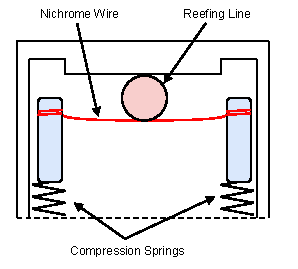
\includegraphics[width=8cm]{images/nichrome-wire}
	\caption{Nichrome wire concept (side view, in line with reefing line)}
	\label{fig:nichrome-wire}
\end{figure}

Initial testing showed that a nichrome wire could burn through a polyamide rope quickly and reliably. Unfortunately, a problem was observed when the reefing line lacked tension. The line would still burn through but melt back together immediately after. The line would stay attached with the nichrome wire out of the way. To combat that, some mechanism is needed to always tension the line. At this point, other thermal options were investigated.

\newpage

\subsubsection{Ceramic Heating Element}
After a long search, commercially available tubular heating elements were discovered. The designed use case for these elements is unknown, but there is some indication that they are being used in electronic cigarettes. The elements are rated to operate at up to 700\,$^\circ$C. The tubular heating element combats all drawbacks from the nichrome wire concept described above \ref{nichrome-wire}. The element's shape allows the rope to move around without transferring force to the heating element.
Additionally, the problem of the wire melting back together is mitigated. However, one of the main drawbacks of the heating element is the high power consumption and the relatively slow temperature rise. Another challenge is that the heating element requires a large voltage and current to be operated.

\begin{figure}[h!]
	\centering
	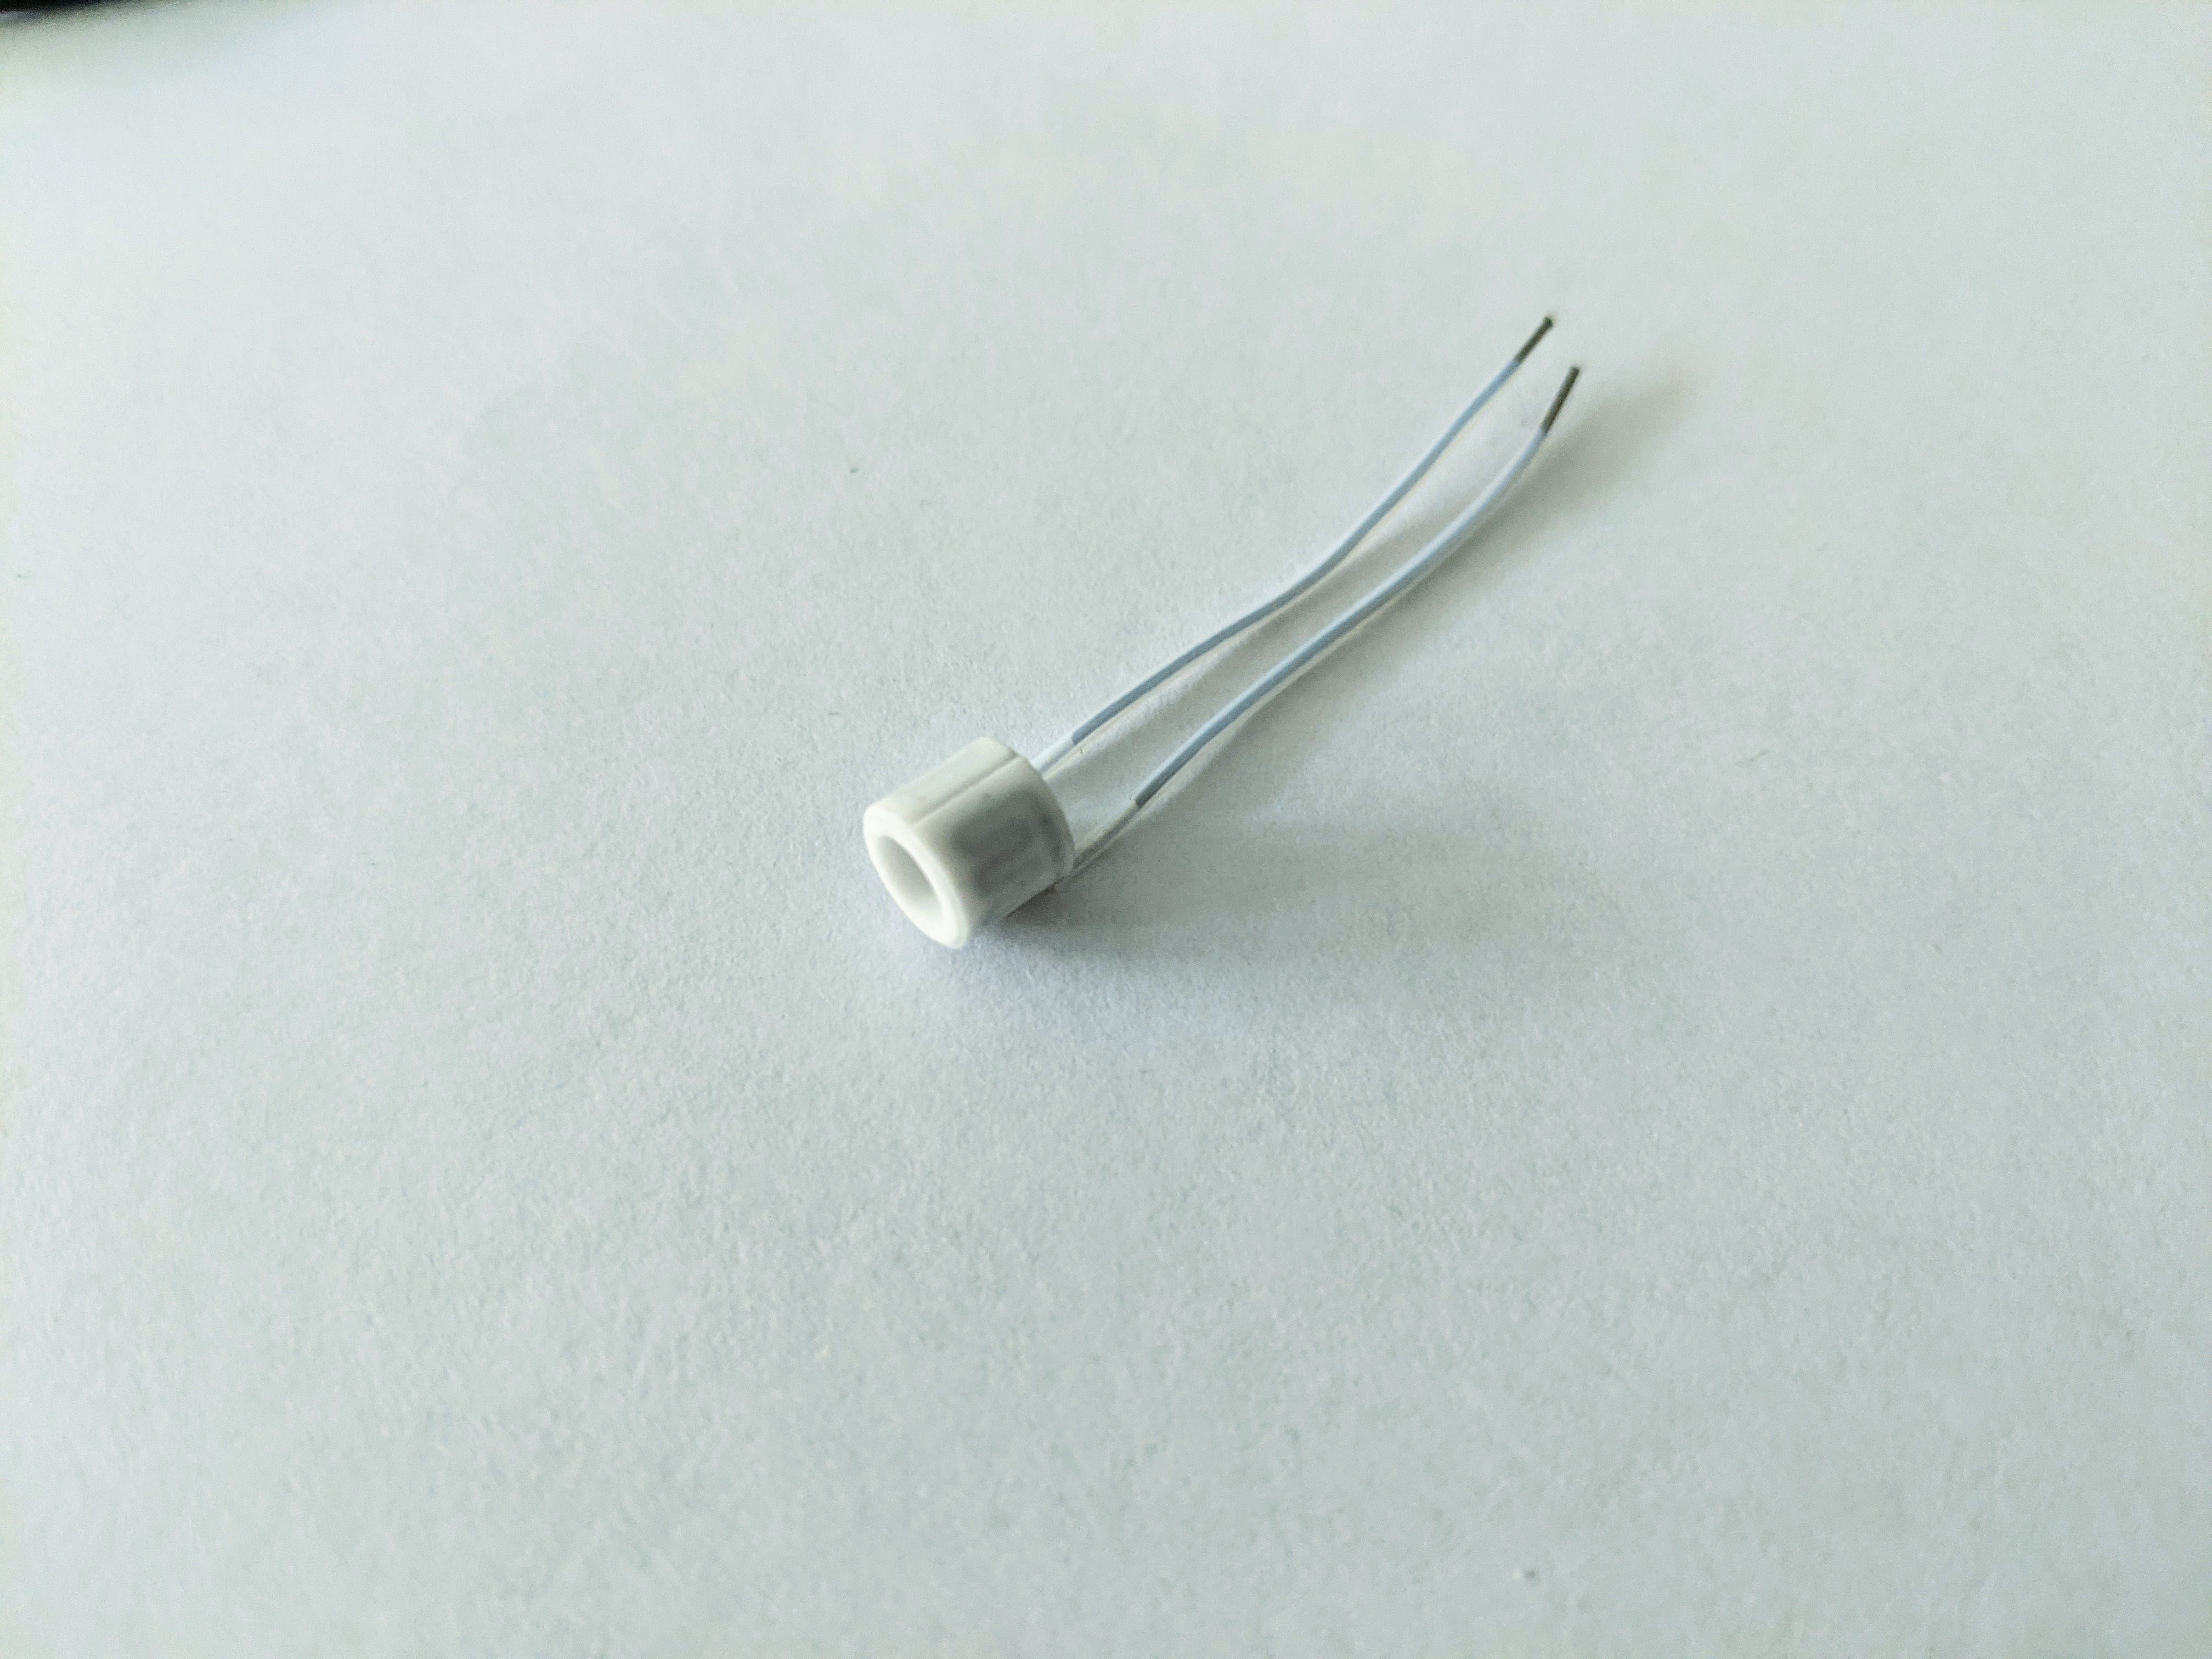
\includegraphics[width=10cm]{images/element}
	\caption{Ceramic Heating element}
	\label{fig:element}
\end{figure}

\newpage

\section{Comparison of Cutting Methods}
A list was created to assess the different cutting methods and decide on a solution. The list was created using the author's limited knowledge, and testing of the different systems and should not be taken as a fact. Especially the reliability is arbitrary and can not be fully assessed before building it. In general, both the electro-mechanical and nichrome wire concepts are medium to low in terms of reliability because the reefing line's force is transferred to the mechanism.  
\begin{table}[h]
    \centering
    \begin{tabular}{ | l | p{2cm} | p{2cm} | p{2cm} | p{1.95cm} |}
      \hline
      \textbf{Method}               & \textbf{Reliability}  & \textbf{Size}  & \textbf{Weight}  & \textbf{Reusable}   \\ \hline
      Servo actuated                & Medium                & Medium         & Medium           & Yes                       \\ \hline
      Linear Solenoid Actuator      & Medium                & Medium         & Medium           & Yes                       \\ \hline
      Continuous Disreefing         & Low                   & Large          & Heavy            & Yes                       \\ \hline
      Pyrotechnic cutter            & Excellent             & Medium         & Medium           & No                        \\ \hline
      Nichrome Wire                 & Medium                & Small          & Light            & Yes                       \\ \hline
      Ceramic Heating Element       & High                  & Small          & Light            & Yes                       \\ \hline
    \end{tabular}
    \caption{\label{tab:cutting-methods}Overview of important line cutter properties}
\end{table}

As shown in Table \ref{tab:cutting-methods}, the pyrotechnic cutter and ceramic heating element are the only two methods that stand out as promising. If the system should be as reliable as possible, pyrotechnic cutters should always be used. However, for this work, reusability was considered more important. Therefore the ceramic heating element cutting method was persuaded.